\documentclass[aip, jmp, amsmath,amssymb, reprint]{revtex4-1}
\usepackage{amsfonts, amssymb, amsthm, pgfplots, array}
\usepackage[thinlines]{easytable}
\usepackage{longtable}
\usepackage{amsmath, mathtools, listings}
\usepackage{graphicx, tikz, }% Include figure files
\usetikzlibrary{arrows, decorations.markings, fit, positioning, shapes}
\tikzset{box/.style={draw, minimum size=2em, text width=20em, text centered},
         bigbox/.style={draw, inner sep=1pt,label={[shift={(-3ex,3ex)}]south east:#1}}
}

\tikzset{main node/.style={circle,draw,minimum size=1cm,inner sep=0pt},}
\tikzset{min node/.style={circle,draw,minimum size=0.5cm,inner sep=0pt},}

 %----------New special chars of computer scientists----------%
\DeclarePairedDelimiter\ceil{\lceil}{\rceil}
\DeclarePairedDelimiter\floor{\lfloor}{\rfloor} 
\newcommand{\N}{\mathbb{N}}
\newcommand{\R}{\mathbb{R}}
\newcommand{\Z}{\mathbb{Z}}

\theoremstyle{definition}
\newtheorem{defn}{Definition}[section]
\newtheorem{exmp}{Example}[section]

% Set font to Computer Modern Sans Serif
\renewcommand*\rmdefault{cmss}

%--------------------------Document--------------------------%
\begin{document}
\title{COS 485 Crib Notes}
\author{Midterm 2}
\maketitle
\section{Formula You Should Know Already}
\begin{align*}
    \sum\limits_{x = 0}^{n} x &= 1 + 2 +....+n-1 + n = (n+1)\left(\frac{n}{2}\right)\\
    \sum\limits_{x = 0}^{\infty} \left(\frac{1}{2}\right)^x &= \frac{1}{1} + \frac{1}{2} + \frac{1}{4} + \frac{1}{8}.... = 2\\
    \sum\limits_{i = 0}^{\ceil{\lg n}} \frac{n}{2^i} &= \frac{n}{1} + \frac{n}{2} + \frac{n}{4} + \frac{n}{8}.... = 2n-1\\
    \sum\limits_{i = 0}^{n} r^i &= \frac{1-r^{n+1}}{1-r}\\
    \frac{n(n+1)(2n+1)}{6} &= 1^2 + 2^2 + 3^3 +...+ (n-1)^2 + n^2\\
    \binom{n}{k} &= \binom{n - 1}{k - 1} + \binom{n - 1}{k}\\
    \lg x &= k\text{, where } 2^k = x\\
    \lg(a^b+ &= b \lg a\\
    a^{\lg b} &= b^{\lg a}\\
    \lg(n!) &= n \lg (n) 
\end{align*}

\section{Time Complexity}
Just a quick refresher. Featured below is an analysis for Selection Sort.\\
\begin{tabular}{c c c c c c c c | c}
\multicolumn{7}{l}{Inner loop iterations:} & & Total\\
\hline
0 & 1 & 2 & 3 & 4 & 5 &...& n-1 & n-1\\
    & 1 & 2 & 3 & 4 & 5 &... & n-1 & n-2\\
    &   & 2 & 3 & 4 & 5 &... & n-1 & n-3\\
    &   &   & 3 & 4 & 5 &... & n-1 & n-4\\
    &   &   &   & 4 & 5 &... & n-1 & n-5\\
    &   &   &   &   & 5 &... & n-1 & n-6\\
    &   &   &   &   &   &... & n-1 & .\\
    &   &   &   &   &   &... & n-1 & .\\
    &   &   &   &   &   &... & n-1 & .\\
    &   &   &   &   &   &... & n-1 & 3\\
    &   &   &   &   &   &... & n-1 & 2\\
    &   &   &   &   &   &... & n-1 & 1\\
\end{tabular}\\
This is is $T(n) = \dfrac{n^2}{2} - \dfrac{n}{2}$, or $O(n^2)$.\\

\section{Order Notation}
\begin{defn}
    For a given complexity function $f(n)$, $O(f(n))$ is the set of complexity functions $g(n)$ for which there exists some real positive constant $c$ and some non-negative integer $N$ s.t. $\forall n \geq N$, $g(n) \leq c \times f(n)$\\
    This means, for example, $\{n^2, 5n + 2, n\lg n ...\}\in O(n^2)$
\end{defn}
\begin{exmp}
\textbf{Show that $n \in O(n^2)$.}\\
By definition, $n \leq c\cdot n^2$. This is true starting at $c = 1$, $N = 1$: $1 \leq 1\cdot n$.
\end{exmp}
\begin{defn}
    $\Omega(f(n))$ is the set of complexity functions $g(n)$ for which there exists some real positive constant $c$ and some non-negative integer $N$ s.t. $\forall n \geq N$, $g(n) \geq c \times f(n)$\\
    This means, for example, $\{n^2, n^3, 2^n ...\}\in \Omega(n^2)$
\end{defn}
\begin{defn}
    $\Theta(f(n)) = O(f(n)) \cap \Omega(f(n))$, meaning it is the set of complexity functions $g(n)$ where there exists some real positive constants $c$, $d$ and some non-negative integer $N$ s.t. $\forall n \geq N$, $c\times f(n) \leq g(n) \leq d \times f(n)$\\
    This means, for example, $\{n^2, 4n^2, n^2 + n\lg n ...\}\in \Theta(n^2)$
\end{defn}
\begin{defn}
    $o(f(n))$ is the set of complexity functions $g(n)$ satisfying the following: $\forall c \in \R^+, \exists N \in Z^+$ s.t. $\forall n \geq N$, $g(n) \leq c \times f(n)$.\\
    This means, for example, $\{n, 5n + 2, n\lg n ...\}\in O(n^2)$.
\end{defn}
\begin{exmp}
\textbf{Show that $n \in o(n^2)$.}\\
By definition, $n \leq c\cdot n^2$. To find a working expression that conforms to our definition, we note $\dfrac{1}{c} \leq n$, meaning this holds for any $N \geq \dfrac{1}{c}$.
\end{exmp}
\begin{exmp}
\textbf{Show that $n \notin o(5n)$.}\\
Use a proof by contradiction. Let $c = \dfrac{1}{6}$. If $n \in o(5n)$, there must exist some $N$ such that, for $n \geq N$, $n \leq \dfrac{1}{6}5n$. This reduces to $1 \leq \dfrac{5}{6}$, which cannot be true.
\end{exmp}
\section{Divide and Conquer}
\begin{longtable}{p{2cm} p{7cm} }
    \textbf{Binary Search} & 
    \parbox[t]{6cm}{Recurrence equation: We halve our problem every step, and make one comparison on each level. This is
    $W(n) = W\left(\dfrac{n}{2}\right) + 1$ for $n > 1$, $n$ a power of 2. $W(1) = 1$.\\
    The solution is $\lg n + 1$ if $n$ is a power of 2, or $\floor{\lg n} + 1$ otherwise.}\\
    \textbf{Mergesort} & \parbox[t]{6cm}{
    Recurrence equation: We split our array in half, mergesort both halves, and then merge the results together.
    $W(n) = 1 + 2W\left(\dfrac{n}{2}\right) + n-1$. $W(1) = 1$\\
    This is $(\ceil{\lg n} + 1)n$, or $\Theta(n\lg n)$.}\\
    \textbf{Quicksort:} & \parbox[t]{6cm}{
    \textit{(Best-case)}\\
    Recurrence equation: We partition our array on a pivot, quicksort both partitions, and we're done. In the best case, our partition is separates the array such that it is divided in half.
    $B(n) = n + 2B\left(\dfrac{n}{2}\right) + 0$. $B(1) = 1$\\
    \textit{(Worst-case)}\\
    Array is sorted in nondecreasing order. We sort the left subarray, then the right, then partition with a cost of:
    $W(n) = W(0) + W\left(n - 1\right) + n - 1 = W\left(n - 1\right) + n - 1$. $W(1) = 1$\\
    As we keep reducing our problem size by one from $n-1$ to $n-2$, $n-3$..., this is $\dfrac{n(n-1)}{2}$.
    }
\end{longtable}
 
\section{Dynamic Programming}
\begin{tabular}{p{2cm} p{6cm} }
    \textbf{Floyd's}\\ \textbf{Algorithm:} & I know this one by heart, (un)fortunately. This uses the matrices $D^(0)$...$D^(n)$ to provide $n^2$ answers in $n^3$ time.\\
    \textbf{Matrix Chain Multiplication:} &
    \parbox[t]{6cm}{Base form: $A_1[d_0\times d_1] \cdot A_2[d_1\times d_2] => R[d_0 \times d_2]$.\\
    Not all orders of multiplication are equivalent. Consider the following:\\
    $A_1[50\times 10] \cdot A_2[10\times 30] \cdot A_2[30\times 20]$\\
    $(A_1\cdot A_2)A_3 = 50\times 10\times 30 + 50\times 30\times 20 = 15000 + 30000$\\
    $A_1(A_2\cdot A_3) = 10\times 30\times 20 + 50\times 10\times 20 = 6000 + 10000$}\\
\end{tabular}

We can use dynamic programming in an $n^3$ algorithm to find the minimum number of multiplications for any given number of matrices. Shown is the setup for matrices $A_1$...$A_5$.
\begin{center}
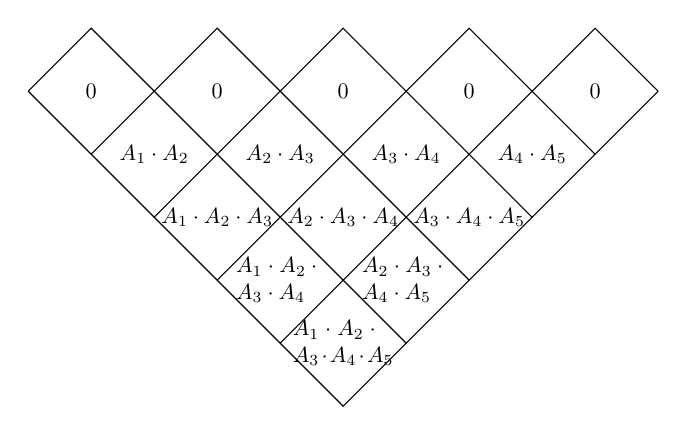
\begin{tikzpicture}[scale = 0.8, every node/.style={scale=0.8}]
    \draw (0,0) -- (5, -5) -- (10, 0)
          (0, 0) -- (1, 1) -- (6, -4)
          (1, -1) -- (3, 1) -- (7, -3)
          (2, -2) -- (5, 1) -- (8, -2)
          (3, -3) -- (7, 1) -- (9, -1)
          (4, -4) -- (9, 1) -- (10, 0);
    \draw (1, 0) node {$0$}
          (3, 0) node {$0$}
          (5, 0) node {$0$}
          (7, 0) node {$0$}
          (9, 0) node {$0$}
          (2, -1) node {$A_1 \cdot A_2$}
          (4, -1) node {$A_2 \cdot A_3$}
          (6, -1) node {$A_3 \cdot A_4$}
          (8, -1) node {$A_4 \cdot A_5$}
          (3, -2) node {$A_1 \cdot A_2 \cdot A_3$}
          (5, -2) node {$A_2 \cdot A_3 \cdot A_4$}
          (7, -2) node {$A_3 \cdot A_4 \cdot A_5$}
          (4, -3) node [text width=1.4cm] {$A_1 \cdot A_2 \cdot A_3 \cdot A_4$}
          (6, -3) node [text width=1.4cm] {$A_2 \cdot A_3 \cdot A_4 \cdot A_5$}
          (5, -4) node [text width=1.6cm] {$A_1 \cdot A_2 \cdot A_3 \cdot A_4 \cdot A_5$};
\end{tikzpicture}
\end{center}
\begin{tabular}{p{2cm} p{6cm} }
    \textbf{Sequence Alignment:} & You know how this works. Pull from the bottom diagonal. Assume a penalty of 1 for a mismatch and a penalty of 2 for a gap, use the dynamic programming algorithm to find an optimal alignment of the following sequences.
\end{tabular}\\
As an example from the last homework:
\begin{center}
    C C G G G T T A C C A\\
    G G A G T T C A
\end{center}
Show both the table and the optimal alignment.
\begin{center}
\begin{tabular}{|cc|c|c|c|c|c|c|c|c|c|c|c|c|}
    \hline
    & \textit{j} & 0 & 1 & 2 & 3 & 4 & 5 & 6 & 7 & 8 & 9 & 10 & 11\\
    \textit{i}& & C & C & G & G & G & T & T & A & C & C & A & \_\\
    \hline
    0 & G & \textbf{8} & \textbf{6} & 5 & 4 & 6 & 7 & 8 & 9 & 11 & 12 & 14 & 16\\
    \hline
    1 & G & 9 & 7 & \textbf{5} & 5 & 4 & 6 & 6 & 7 & 9 & 10 & 12 & 14\\
    \hline
    2 & A & 11 & 9 & \textbf{7} & 5 & 5 & 4 & 5 & 5 & 7 & 8 & 10 & 12\\
    \hline
    3 & G & 12 & 10 & 8 & \textbf{6} & \textbf{4} & 4 & 3 & 4 & 5 & 6 & 8 & 10\\
    \hline
    4 & T & 14 & 12 & 10 & 8 & 6 & \textbf{4} & 3 & 2 & 3 & 4 & 6 & 8\\
    \hline
    5 & T & 16 & 14 & 12 & 10 & 8 & 6 & \textbf{4} & 3 & 1 & 2 & 4 & 6\\
    \hline
    6 & C & 18 & 16 & 14 & 12 & 10 & 8 & 6 & \textbf{4} & \textbf{2} & \textbf{0} & 2 & 4\\
    \hline
    7 & A & 20 & 18 & 16 & 14 & 12 & 10 & 8 & 6 & 4 & 2 & \textbf{0} & 2\\
    \hline
    8 & \_ & 22 & 20 & 18 & 16 & 14 & 12 & 10 & 8 & 6 & 4 & 2 & \textbf{0}\\
    \hline
\end{tabular}
\end{center}

\section{Minimum Spanning Trees and Greedy Algorithms}
\begin{longtable}{p{2cm} p{6cm} }
    \textbf{Spanning Tree} & For a graph $G$, it's spanning tree is a connected subgraph that contains all of $G$'s verticies and is a tree.\\
    \textbf{Minimum}\\ \textbf{Spanning Tree} & For a graph $G$, it is a spanning tree of minimum weight.\\\\
    \textbf{Prim's}\\ \textbf{Algorithm} & Builds a minimum spanning tree vertex by vertex using an arbitrary starting vertex. Each step it will add the cheapest possible connection from the current vertex to the next. The algorithm is $\Theta(n^2)$.\\
    \textbf{Kruskal's}\\ \textbf{Algorithm} & \parbox[t]{6cm}{
    Builds a minimum spanning tree edge by edge, taking the cheapest edge available unless it causes a cycle. The steps to implement are as follows:
    \begin{enumerate}
        \item Sort the edges in time $\Theta(E \lg(E))$.
        \item Loop through the list of edges for a candidate edge. In worst case, it is $\Theta(E)$.
    \end{enumerate}
    In the worst case, though, every vertex is connected to every other vertex. This means $E \in \Theta(V^2)$. Thus, the worst case complexity is $\Theta((V^2 \lg(E))$.
    }
\end{longtable}
From the above descriptions, we can quickly conclude that Kruskal's Algorithm is better for sparse graphs, and Prim's Algorithm is better for dense graphs.
\begin{longtable}{p{2cm} p{6cm} }
    \textbf{Dijkstra's}\\ \textbf{Algorithm} & \parbox[t]{6cm}{
    Builds a shortest path from a vertex $v_0$ to a destination $v_n$ vertex by vertex using an arbitrary starting vertex. Each step it will add the cheapest possible connection from the tree to another vertex, \textit{using the available connections already made in order to reduce possible costs}. The algorithm is $\Theta(n^2)$.
    }
\end{longtable}

\section{Backtracking}
Note that the book explicitly states that backtracking is a modification of DFS. We just DFS a lot.\\
You remember DFS. Recall the following?
\textit{Demonstrate the use of depth first search on this graph starting at vertex A. Draw the search tree and number the vertices in the order they are first encountered.}
\begin{center}
    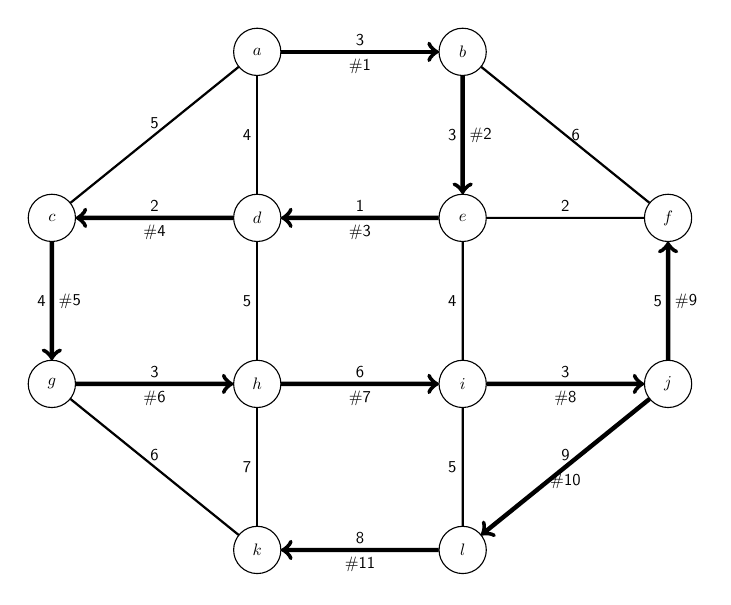
\begin{tikzpicture}[scale = 0.6, every node/.style={scale=0.6}]
       \node[main node] (1) {$a$};
       \node[main node] (2) [right = 2cm of 1]{$b$};
       
       \node[main node] (3) [below = 1.5cm of 1]{$d$};
       \node[main node] (4) [below = 1.5cm of 2]{$e$};
       \node[main node] (5) [left = 2cm of 3]{$c$};
       \node[main node] (6) [right = 2cm of 4]{$f$};
       
       \node[main node] (7) [below = 1.5cm of 5]{$g$};
       \node[main node] (8) [below = 1.5cm of 3]{$h$};
       \node[main node] (9) [below = 1.5cm of 4]{$i$};
       \node[main node] (10) [below = 1.5cm of 6]{$j$};
       
       \node[main node] (11) [below = 1.5cm of 8]{$k$};
       \node[main node] (12) [below = 1.5cm of 9]{$l$};
       \path[draw,thick]
       (1) edge node [above]{3} (2)
       (1) edge node [left]{4} (3)
       (5) edge node [above]{5} (1)
       (5) edge node [above]{2} (3)
       (3) edge node [above]{1} (4)
       (2) edge node [left]{3} (4)
       (2) edge node [right]{6} (6)
       (4) edge node [above]{2} (6)
       (5) edge node [left]{4} (7)
       (3) edge node [left]{5} (8)
       (4) edge node [left]{4} (9)
       (6) edge node [left]{5} (10)
       (7) edge node [above]{3} (8)
       (8) edge node [above]{6} (9)
       (9) edge node [above]{3} (10)
       (7) edge node [above]{6} (11)
       (8) edge node [left]{7} (11)
       (11) edge node [above]{8} (12)
       (9) edge node [left]{5} (12)
       (10) edge node [above]{9} (12);
       
       \path[draw,ultra thick, ->]
       (1) edge node [below]{\#1} (2)
       (2) edge node [right]{\#2} (4)
       (4) edge node [below]{\#3} (3)
       (3) edge node [below]{\#4} (5)
       (5) edge node [right]{\#5} (7)
       (7) edge node [below]{\#6} (8)
       (8) edge node [below]{\#7} (9)
       (9) edge node [below]{\#8} (10)
       (10) edge node [right]{\#9} (6)
       (10) edge node [below]{\#10} (12)
       (12) edge node [below]{\#11} (11)
       ;
    \end{tikzpicture}
\end{center}
The path taken is ABEDCGHIJFLK.\\
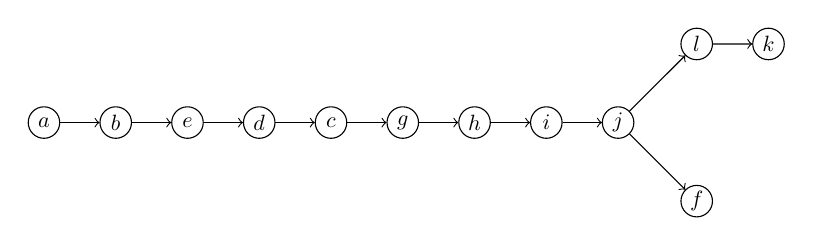
\begin{tikzpicture}[scale = 0.8, every node/.style={scale=0.8}]
   \node[min node] (1) {$a$};
   \node[min node] (2) [right = 0.5cm of 1]{$b$};
   \node[min node] (3) [right = 0.5cm of 2]{$e$};
   \node[min node] (4) [right = 0.5cm of 3]{$d$};
   \node[min node] (5) [right = 0.5cm of 4]{$c$};
   \node[min node] (6) [right = 0.5cm of 5]{$g$};
   \node[min node] (7) [right = 0.5cm of 6]{$h$};
   \node[min node] (8) [right = 0.5cm of 7]{$i$};
   \node[min node] (9) [right = 0.5cm of 8]{$j$};
   \node[min node] (10) [below right = 1cm of 9]{$f$};
   \node[min node] (11) [above right = 1cm of 9]{$l$};
   \node[min node] (12) [right = 0.5cm of 11]{$k$};
   \path[draw, ->]
   (1) edge node {} (2)
   (2) edge node {} (3)
   (3) edge node {} (4)
   (4) edge node {} (5)
   (5) edge node {} (6)
   (6) edge node {} (7)
   (7) edge node {} (8)
   (8) edge node {} (9)
   (9) edge node {} (10)
   (9) edge node {} (11)
   (11) edge node {} (12);
\end{tikzpicture}
    
\begin{longtable}{p{2.2cm} p{6cm} }
        \textbf{DFS} & DFS is a  $\Theta(V + E)$ traversal of any graph. Pseudocode for the recursive form is as follows.
\begin{lstlisting}[language=php]
mark the curr vertex, u, visited
enter u in the discovery order set

foreach vertex, v, adjacent 
to the curr vertex, u:
  if v !visited:
    Set parent of v to u
    DFS starting at v
mark u finished 
enter u in the 'finished' set
    
\end{lstlisting}\\
    \textbf{Backtracking} & Create a state space tree and traverse it. After determining that a node can only lead to death and destruction, go back to the parent and try again. The only way we can determine this is either by running out of options to come up with a solution, or using an upper bound to state a solution will get no worse. These algorithms are pretty terrible; the $n-queens$ problem uses a $\Theta(n^n)$ solution. The sum-of-subsets problem uses an upper bound and is a $T_n \approx 2^{n+1}-1$ algorithm
\end{longtable}
\section{Branch-and-Bound}
Note that the book explicitly states that backtracking is a modification of \textit{breadth}-first search. We just BFS a lot.
\begin{longtable}{p{2.2cm} p{6cm} }
    \textbf{BFS} & BFS is also a  $\Theta(V + E)$ traversal of any graph, using a dequeue.\\
    \textbf{Branch-and-Bound} & Just like Backtracking, with the modification that we visit the children of the current node only if its bound (an estimate guessing what will follow the current node) indicates that that path will lead to a better solution than the current best solution. That's the only effective difference. This is a \textbf{best}-first search.
\end{longtable}

\section{Monte Carlo}

Determines the number of nodes on a search tree. Start at a random staring point and solve the problem as we normally would. Repeat until 
we have either exhausted our search space, or have found a solution.

\begin{center}
\begin{TAB}(e){|c|c|c|c|c|c|c|c|c|}{|c|c|c|c|c|c|c|c|c|}
	$\cdot$ & $\cdot$ & \textcolor{red}{$\mathrm{Q}_1$} & $\cdot$ & $\cdot$ & $\cdot$ & $\cdot$ & $\cdot$ & $\cdot$ \\
	$\cdot$ & $\textcolor{red}{\mathrm{x}_1}$ & $\textcolor{red}{\mathrm{x}_1}$ & $\textcolor{red}{\mathrm{x}_1}$ & $\cdot$ & $\cdot$ & $\cdot$ & $\cdot$ & \textcolor{blue}{$\mathrm{Q}_2$} \\
	$\textcolor{red}{\mathrm{x}_1}$ & \textcolor{green}{$\mathrm{Q}_3$} & $\textcolor{red}{\mathrm{x}_1}$ & $\cdot$ & $\textcolor{red}{\mathrm{x}_1}$ & $\cdot$ & $\cdot$ & $\textcolor{blue}{\mathrm{x}_2}$ & $\textcolor{blue}{\mathrm{x}_2}$ \\
	$\textcolor{green}{\mathrm{x}_3}$ & $\textcolor{green}{\mathrm{x}_3}$ & $\textcolor{red}{\mathrm{x}_1}$ & $\cdot$ & $\cdot$ & $\textcolor{red}{\mathrm{x}_1}$ & $\textcolor{blue}{\mathrm{x}_2}$ &  \textcolor{yellow}{$\mathrm{Q}_4$} & $\textcolor{blue}{\mathrm{x}_2}$ \\
	\textcolor{cyan}{$\mathrm{Q}_5$} & $\textcolor{green}{\mathrm{x}_3}$ & $\textcolor{red}{\mathrm{x}_1}$ & $\textcolor{green}{\mathrm{x}_3}$ & $\cdot$ & $\textcolor{blue}{\mathrm{x}_2}$ & $\textcolor{red}{\mathrm{x}_1}$ & $\textcolor{yellow}{\mathrm{x}_4}$ & $\textcolor{blue}{\mathrm{x}_2}$ \\
	$\textcolor{cyan}{\mathrm{x}_5}$ & $\textcolor{green}{\mathrm{x}_3}$ & $\textcolor{red}{\mathrm{x}_1}$ & \textcolor{teal}{$\mathrm{Q}_6$} & $\textcolor{blue}{\mathrm{x}_2}$ & $\textcolor{yellow}{\mathrm{x}_4}$ & $\cdot$ & $\textcolor{red}{\mathrm{x}_1}$ & $\textcolor{blue}{\mathrm{x}_2}$ \\
	$\textcolor{cyan}{\mathrm{x}_5}$ & $\textcolor{green}{\mathrm{x}_3}$ & $\textcolor{red}{\mathrm{x}_1}$ & $\textcolor{blue}{\mathrm{x}_2}$ & $\textcolor{yellow}{\mathrm{x}_4}$ & $\textcolor{green}{\mathrm{x}_3}$ & \textcolor{magenta}{$\mathrm{Q}_7$} & $\textcolor{yellow}{\mathrm{x}_4}$ & $\textcolor{red}{\mathrm{x}_1}$ \\
	$\textcolor{cyan}{\mathrm{x}_5}$ & $\textcolor{green}{\mathrm{x}_3}$ & $\textcolor{red}{\mathrm{x}_1}$ & $\textcolor{yellow}{\mathrm{x}_4}$ & \textcolor{olive}{$\mathrm{Q}_8$} & $\textcolor{teal}{\mathrm{x}_6}$ & $\textcolor{green}{\mathrm{x}_3}$ & $\textcolor{yellow}{\mathrm{x}_4}$ & $\textcolor{blue}{\mathrm{x}_2}$ \\
	$\textcolor{cyan}{\mathrm{x}_5}$ & $\textcolor{blue}{\mathrm{x}_2}$ & $\textcolor{red}{\mathrm{x}_1}$ & $\textcolor{teal}{\mathrm{x}_6}$ & $\textcolor{cyan}{\mathrm{x}_5}$ & $\textcolor{olive}{\mathrm{x}_8}$ & $\textcolor{teal}{\mathrm{x}_6}$ & $\textcolor{green}{\mathrm{x}_3}$ & $\textcolor{blue}{\mathrm{x}_2}$ \\
\end{TAB}
\end{center}

\begin{center}
\begin{tabular}{l | c | l}
	\textbf{Row \#} & \textbf{Choices} & \textbf{Cost} \\
	1 & 9 & 9 \\
	2 & 6 & $9 \cdot 6$ \\
	3 & 4 & $9 \cdot 6 \cdot 4$ \\
	4 & 3 & $9 \cdot 6 \cdot 4 \cdot 3$ \\
	5 & 2 & $9 \cdot 6 \cdot 4 \cdot 3 \cdot 2$ \\
	6 & 2 & $9 \cdot 6 \cdot 4 \cdot 3 \cdot 2 \cdot 2$ \\
	7 & 1 & $9 \cdot 6 \cdot 4 \cdot 3 \cdot 2 \cdot 2 \cdot 1$ \\
	8 & 1 & $9 \cdot 6 \cdot 4 \cdot 3 \cdot 2 \cdot 2 \cdot 1 \cdot 1$ \\
	9 & 0 & 0 \\
	\hline
	\textbf{Total} & & \textbf{9999}
\end{tabular}
\end{center}

\section{Computational Complexity}

There are three categories of algorithms
\begin{longtable}{p{2.2cm} p{6cm} }
    \textbf{P} & Problems with known polynomial-time solutions \\
    \textbf{NP} & Problems whose solutions can be verified in polynomial time (VP) \\
    \textbf{Intractable} & Problems proven to be unsolvable in polynomial time. This can happen in two waays. Either we produce a
                           non-polynomial amount of output or we can prove that the problem takes exponential time to solve. \\
\end{longtable}

In the set of problems designated \textbf{NP} there are four subcategories
\begin{longtable}{p{2.2cm} p{6cm} }
    \textbf{NP-Complete} & A problem $B$ is called $NP$-complete if both of the following are true. 
                            \begin{enumerate}
                                \item $B \in NP$ 
                                \item For every other problem $A \in NP$, $A \propto B$.
                            \end{enumerate} \\
    \textbf{NP-Easy} & A problem $A$ is called $NP$-easy if, for some problem $B \in NP$ $A \propto_T B$. \\
    \textbf{NP-Hard} & A problem $B$ is called $NP$-hard if, for some $NP$-complete problem $A$. $A \propto_T B$. \\
    \textbf{NP-Equivalent} & A problem is called $NP$-equivalent if it is both $NP$-hard and $NP$-easy. \\
\end{longtable}

In the above we use the operations $\propto$ and $\propto_T$. They are defined below:
\begin{longtable}{p{2.2cm} p{6cm} }
    \textbf{$\propto$} & If there exists a polynomial-time transformation algorithm from decision problem $A$, to decision problem $B$, then
                         problem $A$ is polynomiaal-time many-one reducable to problem $B$. This is $A \propto B$. \\
    \textbf{$\propto_T$} & If a problem $A$ can be solved in polynomial-time with a hypothetical polynomial-time algorithm for problem $B$,
                           then problem $A$ is polynomial-time Turing reducable to problem $B$. This is $A \propto_T B$. \\
\end{longtable}

Examples of Problem Transforms:

\begin{longtable}{p{2.2cm} p{6cm} }
    $P_x \propto P_{\textrm{easy}}$  & $P_x$ is easy \\
    $P_y \propto P_{\textrm{hard}}$  & $P_y$ is unknown \\
    $P_{\textrm{hard}} \propto P_z$  & $P_z$ is hard \\
    $P_{\textrm{easy}} \propto P_a$  & $P_a$ is unknown \\
    $P_1 \propto P_2$ \\ and $P_2 \propto P_1$  & $P_1$ and $P_2$ are both easy or both hard. \\\\
    $P_h,\cdots, P_k$ \\  $\propto P_\pi$  & If $P_\pi$ is hard, then the others are unknown. If $P_\pi$ is easy, then they all are easy.
                                                If any of $ P_h,\, \cdots , \, P_k$ is hard, then $P_\pi$ is hard. \\

\end{longtable}

\section{NP-complete Problems}

There are a famous set of problems which we have discussed in class for which Boothe is fairly sure there is no polynomial-time solution.
\begin{longtable}{p{2.2cm} p{6cm} }
    \textbf{Bin Packing} & Given a set of numbers, how do you pack them into the minimum number of bins with a specified capacity. \\
    \textbf{Subset Sum} & Given a set of numbers, using only one bin, how can you pack the bin as close to capacity as possible without 
                          overflow \\
    \textbf{0-1 Knapsack} & What is the maximum value you can fit in a pack with a specified weight-limit \\
    \textbf{Traveling Salesmen} & Find the shortest path through a weighted graph while visiting all of the nodes. \\\\
    \textbf{Hamiltonian Circuit} & Find a complete tour of a graph. \\
    \textbf{Graph Coloring} & Color a graph such that no two adjacent nodes have the same color with the fewest possible colors. \\
    \textbf{Max Clique} & What is the largest set of verticies all directly connected to one another. \\
    \textbf{Vertex Cover} & Find the smallest set of verticies such that every edge in the graph is attached to a vertex in that set. \\
    \textbf{Satisfiability} & Evaluate if a given statement of boolean logic can ever be true. \\
    \textbf{N-Queens} & Find a placement of $N$ queens on an $N\times N$ board so that no queen threatens another queen. \\
\end{longtable}

\section{Problem Size Expansion}

In order to solve this problem we must define what the Fibonacci sequence is:

\begin{quote}
The Fibonacci sequence, which is discussed in Subsection 1.2.2 is 
defined as follows: 
%
\begin{align*}
t_n &= t_{n-1} + t_{n-2} \\
t_0 &= 0 \\
t_1 &= 1
\end{align*}
This definition gives us the recurrence equation for calculating the $n$th 
term in the Fibonacci sequence, regardless of implementation.
\end{quote}
%
$$
t_n = 
    \dfrac{\left[\dfrac{1 + \sqrt{5}}{2}\right]^n - 
           \left[\dfrac{1 - \sqrt{5}}{2}\right]^n}{\sqrt{5}}
$$
This is clearly not a polynomial. Also, this recurrence equation gives us a 
representation of the amount of output produced by this algorithm and not the
time complexity. 
\\
\\
Even though we subtract one exponential from another, as $n \rightarrow \infty$
the second term approaches zero as $\frac{1 - \sqrt{5}}{2} < 1$. Thus we
are left with a single exponential term. This means that the output produced
is non-polynomial in $n$.
\\
\\
The size of the input to this problem is not $n$, but rather is $2^d$ if we 
assume a binary representation scheme for numbers. $d$ is the number of binary
digits, which is defined by the text as the input size. Solving $n = 2^d$ for 
$d$ gives us $d = \floor{\lg(n)} + 1$. Thus our equation for the amount of 
output produced to represent the $n$th term in the Fibonacci sequence is 
$$
t_n = 
    \dfrac{\left[\dfrac{1 + \sqrt{5}}{2}\right]^{2^d} - 
           \left[\dfrac{1 - \sqrt{5}}{2}\right]^{2^d}}{\sqrt{5}}
$$
Thus the amount of output produced in representing the $n$th term in the 
Fibonacci sequence is non-polynomial with respect to $d$, where $d$ is the input 
size. Thus this problem is inherently intractable by definition as it produces
a non-polynomial amount of output.

\section{Transformation Complexity Augmentation}

We are given two problems $A$, $B$, such that $A$ can be converted to $B$ in 
$t_n \in \Theta(n^a) \in P$ where $P$ is the set of all polynomials. Thus 
$A \propto B$. We also note that $B$ is solvable in $t_n \in \Theta(n^b) \in P$.
To bound the complexity of this solution, consider the following:

\begin{proof}
Suppose we have an instance of problem $A$ that is of size $n$. Because at 
most there are $\Theta(n^a)$ steps in the transformation algorithm, and at 
worst the algorithm outputs a symbol at each step, the size of the instance 
of $B$ produced by the transformation is at most a quantity $s$ such that 
$s \in \Theta(n^a)$. 
When $s$ is the input to the algorithm for $B$, there are at most 
$\Theta\left(s^b\right) = \Theta\left((n^a)^b\right) = 
\Theta\left(n^{ab}\right)$ steps. Therefore, 
the maximum number of steps required to transform the instance of problem $A$ 
to an instance of problem $B$ and then solve problem $B$ to get the correct 
answer for problem $A$ is at most
$$
\Theta(n^a) + \Theta\left(n^{ab}\right)
$$
which is a polynomial in $n$.
\end{proof}
\end{document}















































